\section{Model fitting and likelihood analysis}

\begin{figure}
\centering
  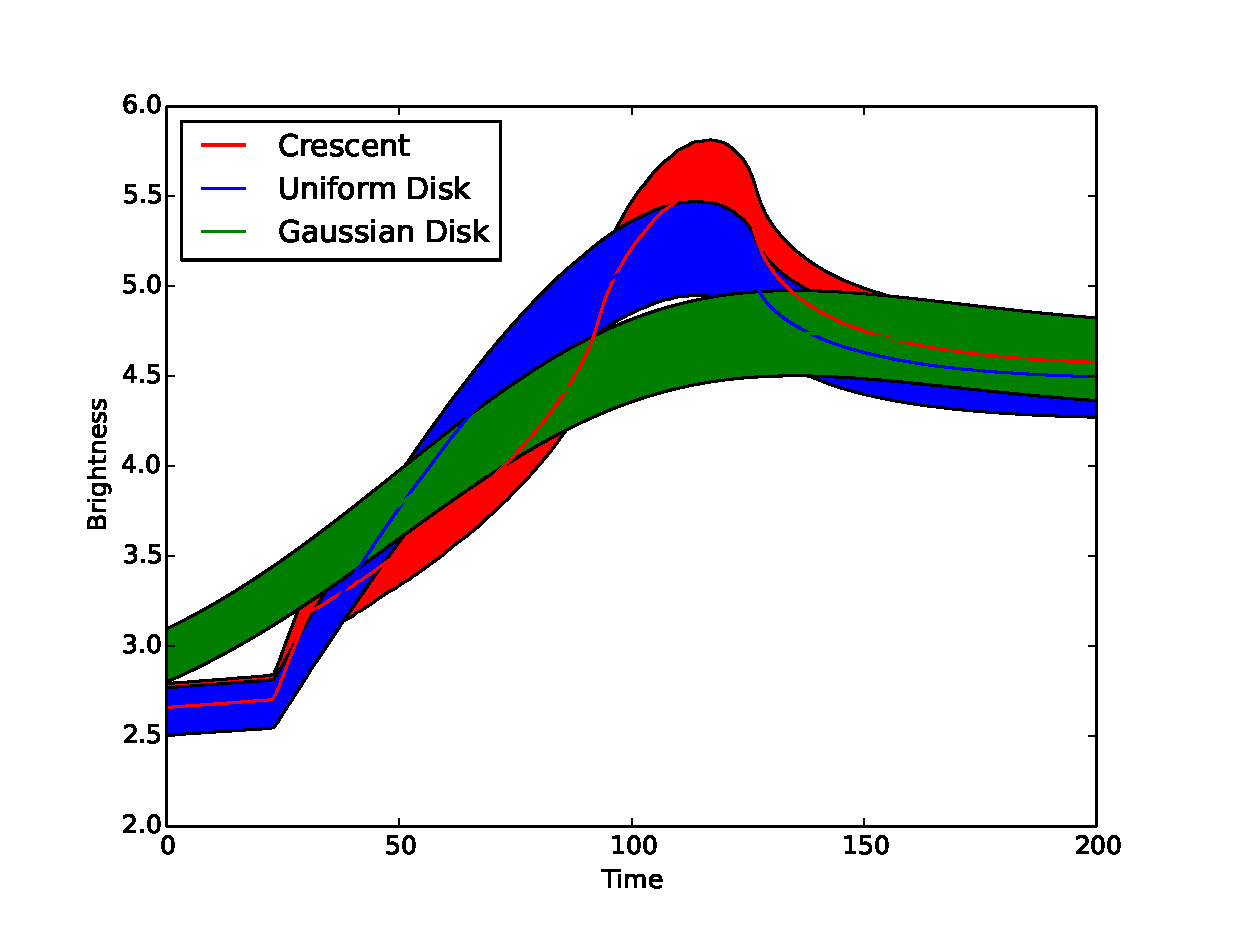
\includegraphics[width=0.95\hsize]{plots/data_with_error.eps}
\caption{\label{fig:datafitting} data}
\end{figure}


\begin{figure}
\centering
  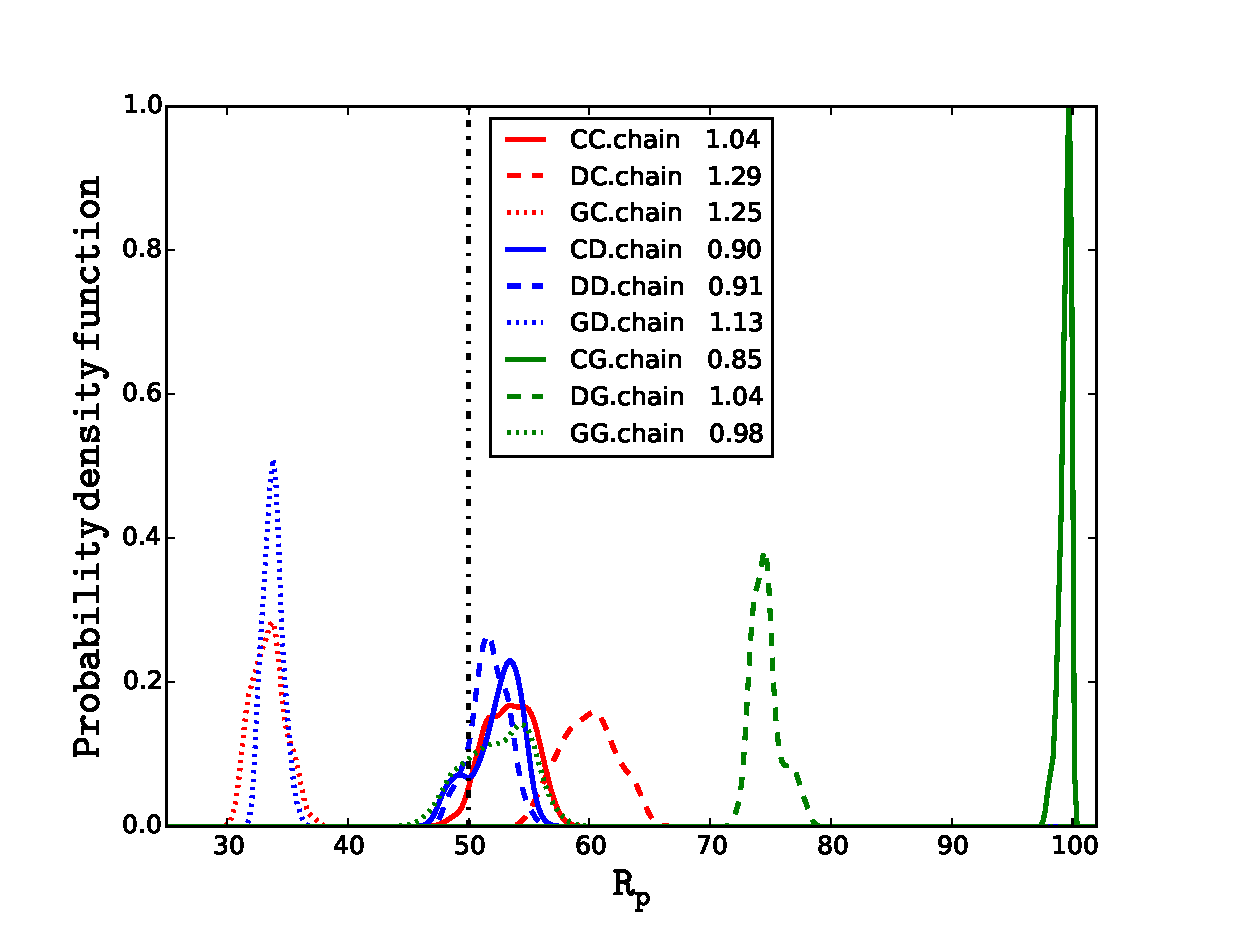
\includegraphics[width=0.45\hsize]{plots/Rp4all.eps}
  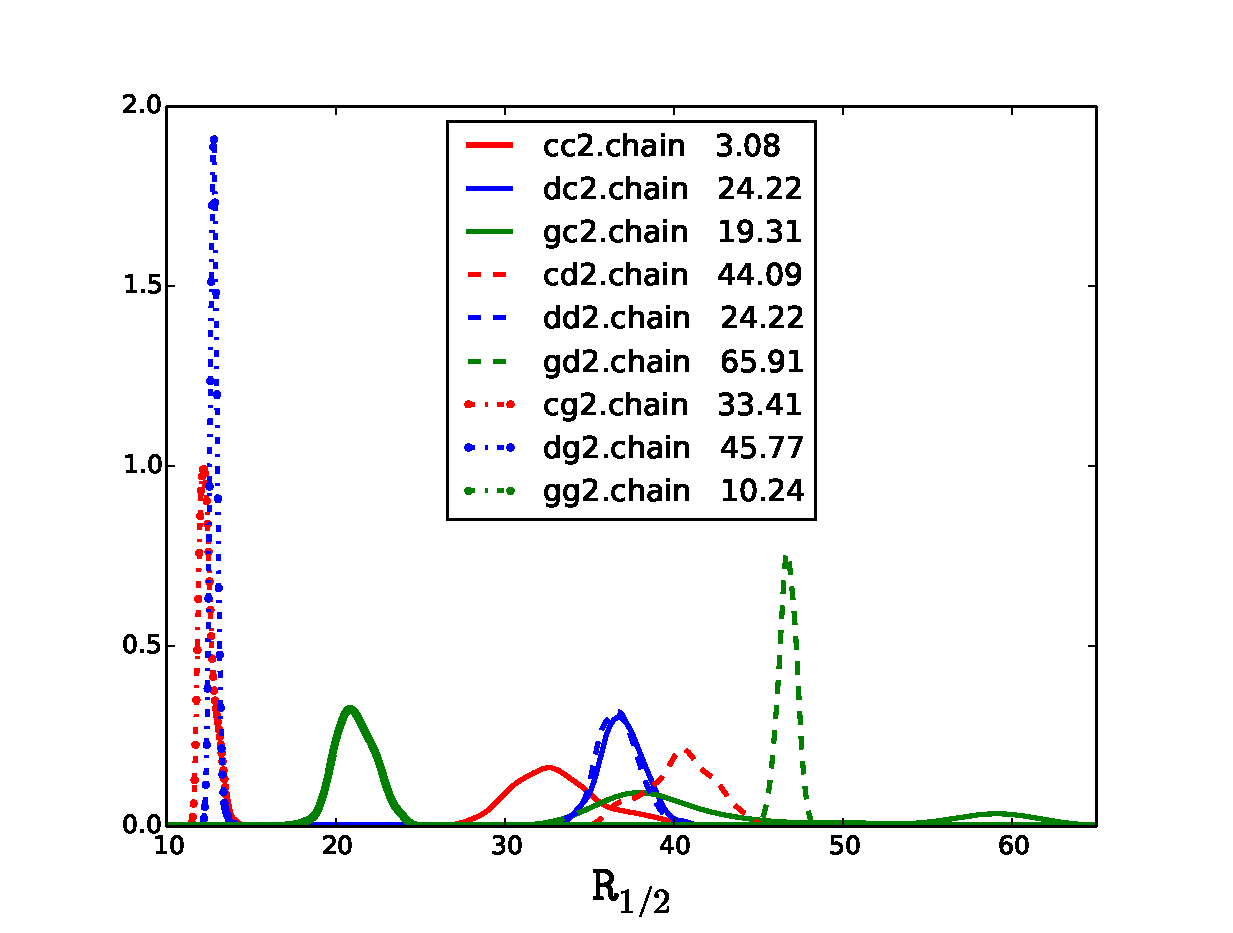
\includegraphics[width=0.45\hsize]{plots/Rhalf4all.eps}\\
  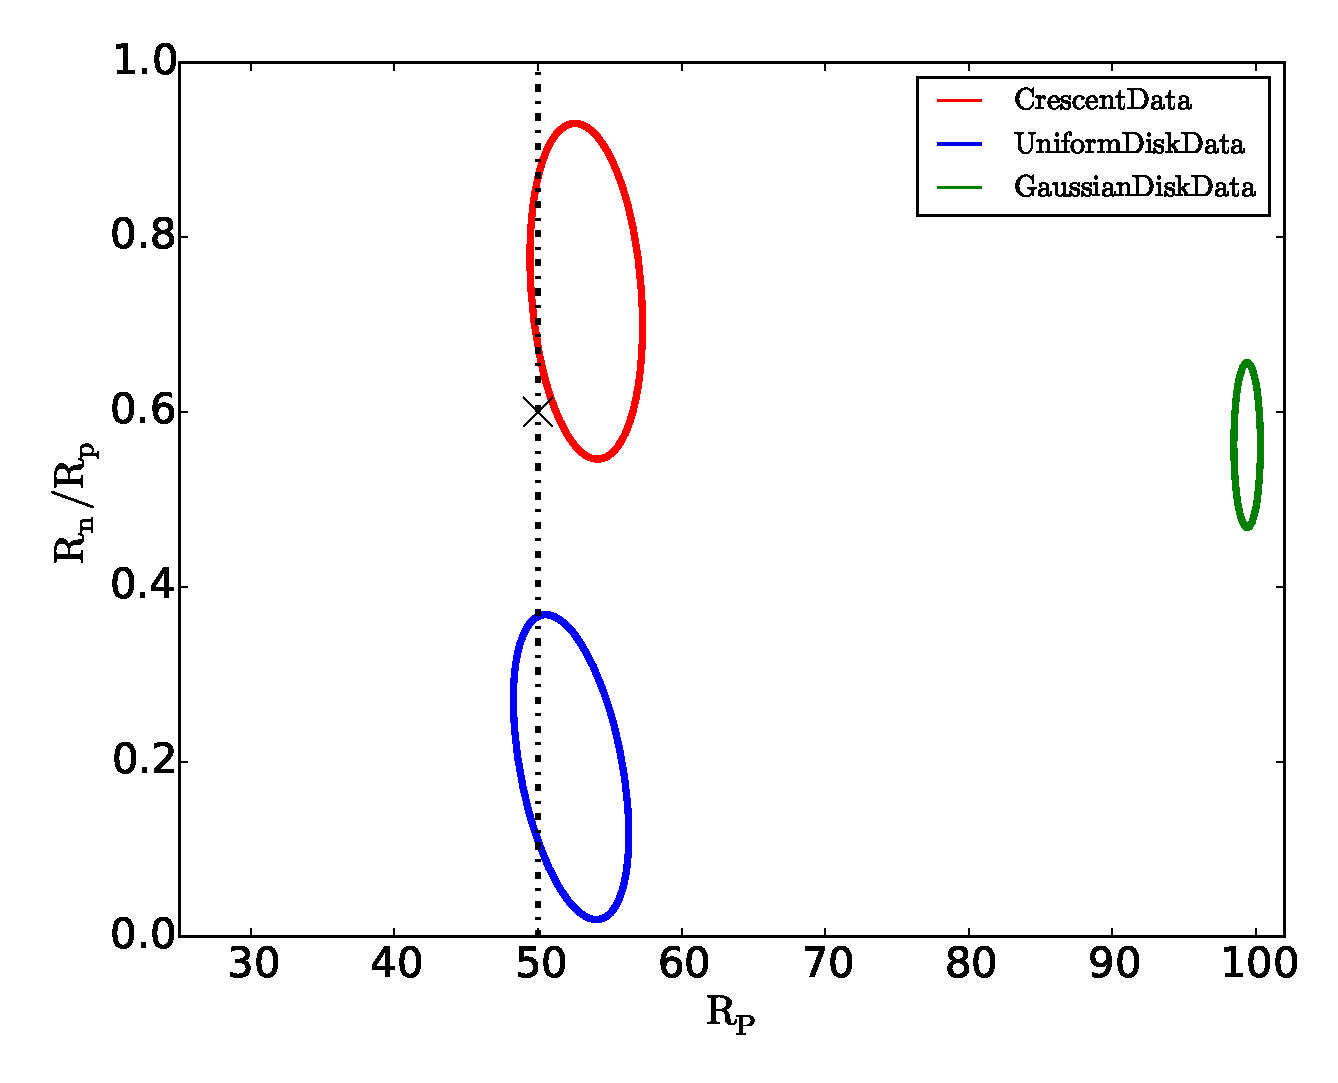
\includegraphics[width=0.45\hsize]{plots/Rhalf_RnRp.eps}
  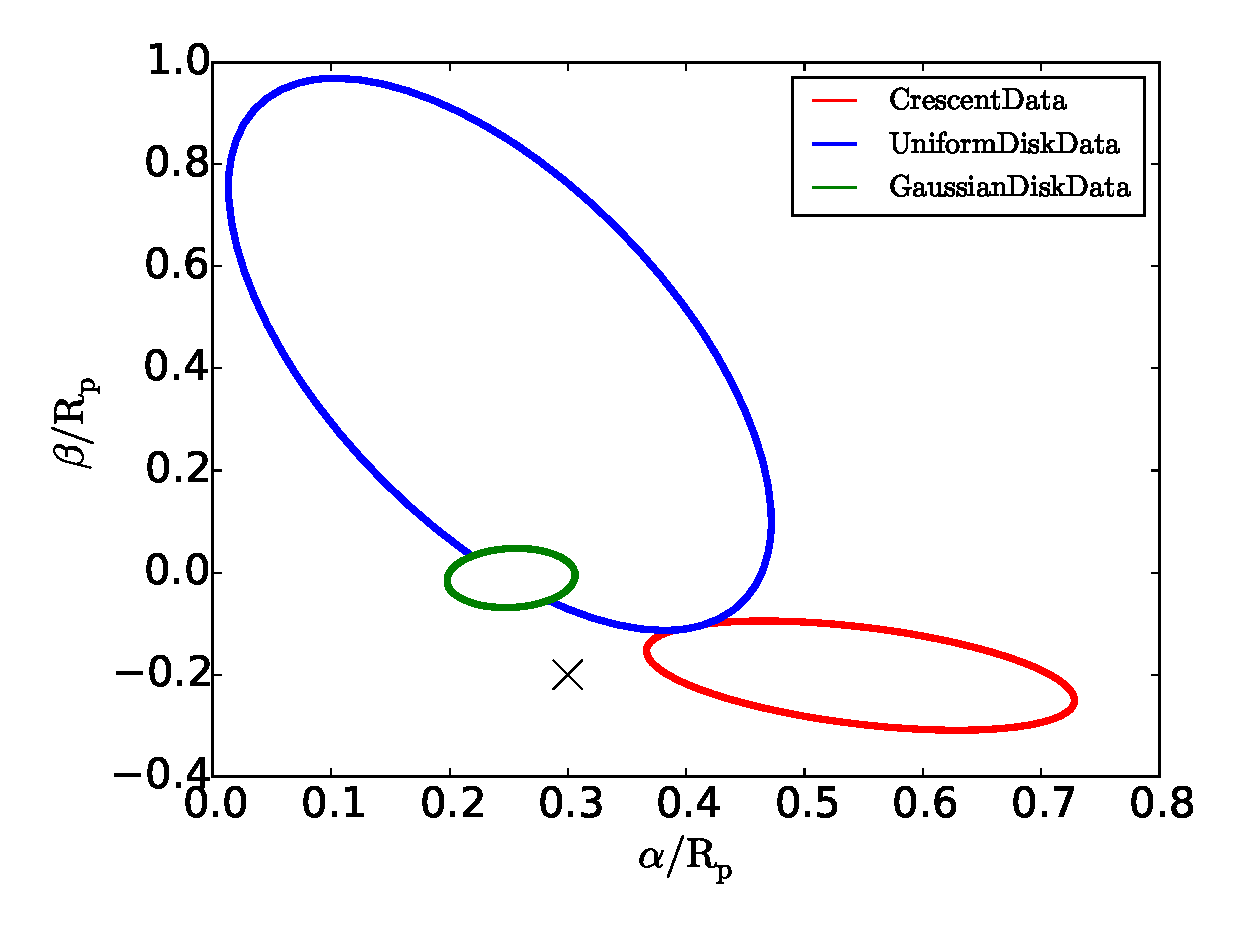
\includegraphics[width=0.45\hsize]{plots/aRp_bRp.eps}

\caption{\label{fig:mcmc} Model Fitting}
\end{figure}


In this section, we attempt to fit and recover the model parameters from the given dataset generated by different source models - crescent, uniform-disk and Gaussian-disk. So broadly we have 9 cases to discuss. We carried out a likelihood analysis on all three parameter set using Markov-chain Monte-Carlo (MCMC). The main results of the MCMC are shown in figure \ref{fig:mcmc}. In the top row, we show the nine curves (likelihood) of recovered size of the source and its half light radius (left and right respectively). The legend of top row plots has information about the datasets, fitting model and best fit. The legend are named as, for example cd.chain, where first alphabet is the dataset and second alphabet is the fitting model. So, cd.chain represents the case where we fit disk model to crescent dataset. The number accompanying the name of the legend is the best fit $-2log(likelihood)$. We follow the convention of red, blue and green color for crescent, uniform disc and Gaussian disk datasets respectively whereas the fitting model is represented by different kind of curves: solid, dashed and dot-dashed respectively.

 In the bottom rows we show three contours, for three different datasets (same color convention) fitted with crescent parameters only because this is the only case with more than one relevant parameter. Note that we plotted the 2D ellipses with principal component analysis of the MCMC and this is the reason they are perfect ellipses and not arbitary shape.

\subsection{Mock datasets}
The datasets for each source model is in the form of light curves, the brightness of the source observed at different time scale. Figure \ref{fig:datafitting} shows the three datasets. These datasets are generated using the magnification map shown in figure \ref{fig:magnification} between point B and C (direction from C to B). The data assumed was very  ideal, including 200 different data points at regular interval of time. It is worth noticing that the datasets generated using crescent model and uniform disc model resembles much more than the one generated by Gaussian disc model source. This is also very intuitive as uniform disc is a special case in crescent model where $R_n=0$. The fiducial model assumed to generate these mock datasets are:
\begin{equation}
	[R_p, R_n, a, b] = [50.0, 30.0, 15.0, 10.0]  \ \ \ \rm{for\ Crescent\ model},
	\label{eqn:cp}
\end{equation}
\begin{equation}
	R = 50.0 \ \ \ \rm{for\ Uniform\ disc\ model}
\end{equation}

\begin{equation}
	R = 50.0 \ \ \ \rm{for\ Gaussian\ disk\ model}
\end{equation}
\\
where, $R$ being the size of the uniform disc and Gaussian disc source model. We also have some nuisance parameters in all these cases: the beginning of the event, the length of the event, normalisation of the lightcurve, however in this analysis, we marginalised over only one nuisance parameter, the beginning of the event, and kept the other two fixed.

The aim of this exercise was to explore the degeneracies in  various model parameters and recover the correct fiducial model assumed. Also, it can be inferred if one can simply distinguish between circularly symmetric and asymmetric sources or uniform and Gaussian sources.
The errorbars on each data point (shaded region in figure \ref{fig:datafitting}), in all three datasets, is about 10 percent its value. Also, because we are fitting these datasets with different (arbitrary) caustic crossing (point A to B in figure \ref{fig:magnification}), it adds a natural systematic errors on each data point. We did not add any random noise to the data points, but because the noise is dominated by the systematic part, in this case, the overall contribution of random noise is negligible. We also assume the errors are Gaussian distributed.


\subsection{Fitting with crescent model}
First we explored the parameter space for crescent source model and run its likelihood exploration for three different datasets. Here we have four parameters as given by equation \ref{eqn:cp}. Three solid curves in top row of figure \ref{fig:mcmc} represents the resulting likelihood of $R_p$, the overall size of the crescent source for three different datasets. Solid red curve in top row and red contours in bottom row of figure \ref{fig:mcmc} represents the crescent fitting with crescent data (cc.chain in figure \ref{fig:mcmc}). All four parameters can be well recovered in this case and the overall likelihood coincides well with the fiducial values assumed and stated in equation \ref{eqn:cp}. It can also be well noticed that the half light radius is degenerate with $R_n/R_p$ or in other words, $R_p$ and $R_n$ are correlated. This degeneracy is not very strong, partially broken, and can be further broken by precise measurements of the light curve. Also, parameters $a$ and $b$ have changed their sign (but almost at the correct numerical value), this is due to fitting a reverse light curve in an opposite direction. These two parameters shows much stronger degeneracy.

In second case, we tried to fit crescent model to disk data (dc.chain in figure \ref{fig:mcmc}). The solid blue in top row and blue contours in bottom row represents this case. Here one can recover the overall shape of the source, slightly lower than what is recovered in cc.chain case. Infact, the likelihood is higher than the previous case as the data is generated by one parameter only and fitting with four parameter that can also model the noise as well. Also, the maximum likelihood is achieved close to $R_n = 0$, as already mentioned, this is intuitive as well. The other paramters, $a$ and $b$ are quite arbitary. 

In the third case, Gaussian disc data is fit with crescent model (gc.chain). The solid green line in top row and green contours in bottom row represents this case. In this case, the extent of $R_p$ is broad and the likelihood is smaller than other cases.

Please notice that in top row of figure \ref{fig:mcmc}, the height of the peaks does not represents the likelihood, it is just ensuring that the area under the curve is unity. The likelihood can be estimated from the number in the legend which is the best $-2log(likelihood)$.

\subsection{Fitting with uniform disc model}
In this case, we have only one parameter to fit, the outer radius of the uniform disc with uniform intensity. When fitting with crescent data (dashed red line), the maximum likelihood shifts towards higher values of $R$ as compared to the fiducial value (which was 50). Also the maximum likelihood is very low and the contraints are also very weak. However, when fitting with Gaussian disc (dashed green line), the likelihood is still very low, but the parameter is tightly constrained. The third case is ideal when fitting uniform disc data (dashed blue line), where the constraints are ideal and also co-incide well with the fiducial value assumed and also likelihood is comparatively better. 


\subsection{Fitting with Gaussian disc model}
In the last case, we fit Gaussian disc model to the three datasets (dat-dashed curves in top row of figure \ref{fig:mcmc}). In this case, when fitted with Gaussian disc data, the likelihood coincide with the fiducial value assumed, in other cases the likelihood is away but weak and very well constrained. 


\subsection{Conclusions and interpretations}
The main results of this work is given in figure \ref{fig:mcmc} and described in the previous section. Here we try to interpret those results and conclude the take away message.

Lets assume that an ideal telescope observes a quasar for a long time and we get the lightcurve with good precision and one can clearly see the event of caustic crossing in the light curve. Now one wants to extract the true shape of the source. To comment more specifically, lets assume three cases when the true shape of the source is: crescent, uniform disc and Gaussian disc:

\begin{enumerate}

\item Crescent shape source: if one tries to fit this curve with crescent model, the maximum likelihood will be good and one can recover the true parameters with good precision. In the other two cases, the maximum likelihood will be very bad. Hence this shape can be recovered very well by trusting the maximum likelihood analysis.
\item Uniform disc shape source: if one tries to fit this curve with Gaussian disk model, the likelihood will be very little to disprove it, however, the other two models are inditinguishable with nearly the same likelihood. At this point it does not matter as one can obtain the true result from both disk and crescent model.
\item Gaussian disc shape source: if one tries to fit this curve with uniform disk model or crescent model, again likelihood will discard this choice. Again the maximum likelihood analysis will point towards the best fitted true model.
\end{enumerate}

At this point, we conclude that maximum likelihood analysis can be well trusted in order to recover true shape and recovering the corresponding parameters. This will provide the accurate recovery of the model parameters, however, for more precise recovery, one rely on precise measurements of the lightcurve.

 
